\PassOptionsToPackage{unicode=true}{hyperref} % options for packages loaded elsewhere
\PassOptionsToPackage{hyphens}{url}
%
\documentclass[]{article}
\usepackage{lmodern}
\usepackage{amssymb,amsmath}
\usepackage{ifxetex,ifluatex}
\usepackage{fixltx2e} % provides \textsubscript
\ifnum 0\ifxetex 1\fi\ifluatex 1\fi=0 % if pdftex
  \usepackage[T1]{fontenc}
  \usepackage[utf8]{inputenc}
  \usepackage{textcomp} % provides euro and other symbols
\else % if luatex or xelatex
  \usepackage{unicode-math}
  \defaultfontfeatures{Ligatures=TeX,Scale=MatchLowercase}
\fi
% use upquote if available, for straight quotes in verbatim environments
\IfFileExists{upquote.sty}{\usepackage{upquote}}{}
% use microtype if available
\IfFileExists{microtype.sty}{%
\usepackage[]{microtype}
\UseMicrotypeSet[protrusion]{basicmath} % disable protrusion for tt fonts
}{}
\IfFileExists{parskip.sty}{%
\usepackage{parskip}
}{% else
\setlength{\parindent}{0pt}
\setlength{\parskip}{6pt plus 2pt minus 1pt}
}
\usepackage{hyperref}
\hypersetup{
            pdftitle={Topic 2: Exercise 1},
            pdfauthor={Daniel Alonso},
            pdfborder={0 0 0},
            breaklinks=true}
\urlstyle{same}  % don't use monospace font for urls
\usepackage[margin=1in]{geometry}
\usepackage{color}
\usepackage{fancyvrb}
\newcommand{\VerbBar}{|}
\newcommand{\VERB}{\Verb[commandchars=\\\{\}]}
\DefineVerbatimEnvironment{Highlighting}{Verbatim}{commandchars=\\\{\}}
% Add ',fontsize=\small' for more characters per line
\usepackage{framed}
\definecolor{shadecolor}{RGB}{248,248,248}
\newenvironment{Shaded}{\begin{snugshade}}{\end{snugshade}}
\newcommand{\AlertTok}[1]{\textcolor[rgb]{0.94,0.16,0.16}{#1}}
\newcommand{\AnnotationTok}[1]{\textcolor[rgb]{0.56,0.35,0.01}{\textbf{\textit{#1}}}}
\newcommand{\AttributeTok}[1]{\textcolor[rgb]{0.77,0.63,0.00}{#1}}
\newcommand{\BaseNTok}[1]{\textcolor[rgb]{0.00,0.00,0.81}{#1}}
\newcommand{\BuiltInTok}[1]{#1}
\newcommand{\CharTok}[1]{\textcolor[rgb]{0.31,0.60,0.02}{#1}}
\newcommand{\CommentTok}[1]{\textcolor[rgb]{0.56,0.35,0.01}{\textit{#1}}}
\newcommand{\CommentVarTok}[1]{\textcolor[rgb]{0.56,0.35,0.01}{\textbf{\textit{#1}}}}
\newcommand{\ConstantTok}[1]{\textcolor[rgb]{0.00,0.00,0.00}{#1}}
\newcommand{\ControlFlowTok}[1]{\textcolor[rgb]{0.13,0.29,0.53}{\textbf{#1}}}
\newcommand{\DataTypeTok}[1]{\textcolor[rgb]{0.13,0.29,0.53}{#1}}
\newcommand{\DecValTok}[1]{\textcolor[rgb]{0.00,0.00,0.81}{#1}}
\newcommand{\DocumentationTok}[1]{\textcolor[rgb]{0.56,0.35,0.01}{\textbf{\textit{#1}}}}
\newcommand{\ErrorTok}[1]{\textcolor[rgb]{0.64,0.00,0.00}{\textbf{#1}}}
\newcommand{\ExtensionTok}[1]{#1}
\newcommand{\FloatTok}[1]{\textcolor[rgb]{0.00,0.00,0.81}{#1}}
\newcommand{\FunctionTok}[1]{\textcolor[rgb]{0.00,0.00,0.00}{#1}}
\newcommand{\ImportTok}[1]{#1}
\newcommand{\InformationTok}[1]{\textcolor[rgb]{0.56,0.35,0.01}{\textbf{\textit{#1}}}}
\newcommand{\KeywordTok}[1]{\textcolor[rgb]{0.13,0.29,0.53}{\textbf{#1}}}
\newcommand{\NormalTok}[1]{#1}
\newcommand{\OperatorTok}[1]{\textcolor[rgb]{0.81,0.36,0.00}{\textbf{#1}}}
\newcommand{\OtherTok}[1]{\textcolor[rgb]{0.56,0.35,0.01}{#1}}
\newcommand{\PreprocessorTok}[1]{\textcolor[rgb]{0.56,0.35,0.01}{\textit{#1}}}
\newcommand{\RegionMarkerTok}[1]{#1}
\newcommand{\SpecialCharTok}[1]{\textcolor[rgb]{0.00,0.00,0.00}{#1}}
\newcommand{\SpecialStringTok}[1]{\textcolor[rgb]{0.31,0.60,0.02}{#1}}
\newcommand{\StringTok}[1]{\textcolor[rgb]{0.31,0.60,0.02}{#1}}
\newcommand{\VariableTok}[1]{\textcolor[rgb]{0.00,0.00,0.00}{#1}}
\newcommand{\VerbatimStringTok}[1]{\textcolor[rgb]{0.31,0.60,0.02}{#1}}
\newcommand{\WarningTok}[1]{\textcolor[rgb]{0.56,0.35,0.01}{\textbf{\textit{#1}}}}
\usepackage{graphicx,grffile}
\makeatletter
\def\maxwidth{\ifdim\Gin@nat@width>\linewidth\linewidth\else\Gin@nat@width\fi}
\def\maxheight{\ifdim\Gin@nat@height>\textheight\textheight\else\Gin@nat@height\fi}
\makeatother
% Scale images if necessary, so that they will not overflow the page
% margins by default, and it is still possible to overwrite the defaults
% using explicit options in \includegraphics[width, height, ...]{}
\setkeys{Gin}{width=\maxwidth,height=\maxheight,keepaspectratio}
\setlength{\emergencystretch}{3em}  % prevent overfull lines
\providecommand{\tightlist}{%
  \setlength{\itemsep}{0pt}\setlength{\parskip}{0pt}}
\setcounter{secnumdepth}{0}
% Redefines (sub)paragraphs to behave more like sections
\ifx\paragraph\undefined\else
\let\oldparagraph\paragraph
\renewcommand{\paragraph}[1]{\oldparagraph{#1}\mbox{}}
\fi
\ifx\subparagraph\undefined\else
\let\oldsubparagraph\subparagraph
\renewcommand{\subparagraph}[1]{\oldsubparagraph{#1}\mbox{}}
\fi

% set default figure placement to htbp
\makeatletter
\def\fps@figure{htbp}
\makeatother


\title{Topic 2: Exercise 1}
\author{Daniel Alonso}
\date{November 28th, 2020}

\begin{document}
\maketitle

\hypertarget{importing-libraries}{%
\paragraph{Importing libraries}\label{importing-libraries}}

\begin{Shaded}
\begin{Highlighting}[]
\KeywordTok{library}\NormalTok{(dplyr)}
\KeywordTok{library}\NormalTok{(Rcpp)}
\end{Highlighting}
\end{Shaded}

\hypertarget{importing-data-as-described-by-exercise}{%
\paragraph{Importing data as described by
exercise}\label{importing-data-as-described-by-exercise}}

\begin{Shaded}
\begin{Highlighting}[]
\NormalTok{d <-}\StringTok{ }\KeywordTok{read.csv}\NormalTok{(}\StringTok{"../../datasets/Colleges.csv"}\NormalTok{)}
\end{Highlighting}
\end{Shaded}

\hypertarget{replacing-binary-variable-private-with-1-and-0}{%
\paragraph{Replacing binary variable Private with 1 and
0}\label{replacing-binary-variable-private-with-1-and-0}}

\begin{Shaded}
\begin{Highlighting}[]
\NormalTok{d}\OperatorTok{$}\NormalTok{Private <-}\StringTok{ }\KeywordTok{ifelse}\NormalTok{(d}\OperatorTok{$}\NormalTok{Private }\OperatorTok{==}\StringTok{ "Yes"}\NormalTok{, }\DecValTok{1}\NormalTok{, }\DecValTok{0}\NormalTok{)}
\end{Highlighting}
\end{Shaded}

\hypertarget{selecting-columns}{%
\paragraph{Selecting columns}\label{selecting-columns}}

\begin{Shaded}
\begin{Highlighting}[]
\NormalTok{data <-}\StringTok{ }\NormalTok{d }\OperatorTok\StringTok{ }\NormalTok{dplyr}\OperatorTok{::}\KeywordTok{select}\NormalTok{(}\StringTok{'Private'}\NormalTok{,}\StringTok{'Apps'}\NormalTok{,}\StringTok{'Accept'}\NormalTok{,}\StringTok{'Enroll'}\NormalTok{,}\StringTok{'F.Undergrad'}\NormalTok{)}
\end{Highlighting}
\end{Shaded}

\hypertarget{calculating-covariances}{%
\paragraph{Calculating covariances}\label{calculating-covariances}}

\begin{Shaded}
\begin{Highlighting}[]
\NormalTok{cov_matrix <-}\StringTok{ }\KeywordTok{cov}\NormalTok{(data)}
\NormalTok{cov_matrix}
\CommentTok{#>                   Private          Apps        Accept       Enroll  F.Undergrad}
\CommentTok{#> Private         0.1986559     -745.3552     -519.2042    -235.1942    -1330.764}
\CommentTok{#> Apps         -745.3552439 14978459.5301  8949859.8119 3045255.9876 15289702.474}
\CommentTok{#> Accept       -519.2042169  8949859.8119  6007959.6988 2076267.7627 10393582.435}
\CommentTok{#> Enroll       -235.1942393  3045255.9876  2076267.7627  863368.3923  4347529.884}
\CommentTok{#> F.Undergrad -1330.7637175 15289702.4742 10393582.4355 4347529.8841 23526579.326}
\end{Highlighting}
\end{Shaded}

\newpage

\hypertarget{calculating-correlations}{%
\paragraph{Calculating correlations}\label{calculating-correlations}}

\begin{Shaded}
\begin{Highlighting}[]
\NormalTok{corr_matrix <-}\StringTok{ }\KeywordTok{cov2cor}\NormalTok{(cov_matrix)}
\NormalTok{corr_matrix}
\CommentTok{#>                Private       Apps     Accept     Enroll F.Undergrad}
\CommentTok{#> Private      1.0000000 -0.4320947 -0.4752520 -0.5679078  -0.6155605}
\CommentTok{#> Apps        -0.4320947  1.0000000  0.9434506  0.8468221   0.8144906}
\CommentTok{#> Accept      -0.4752520  0.9434506  1.0000000  0.9116367   0.8742233}
\CommentTok{#> Enroll      -0.5679078  0.8468221  0.9116367  1.0000000   0.9646397}
\CommentTok{#> F.Undergrad -0.6155605  0.8144906  0.8742233  0.9646397   1.0000000}
\end{Highlighting}
\end{Shaded}

\hypertarget{experimenting-a-little-bit-with-the-private-variable}{%
\paragraph{Experimenting a little bit with the private
variable}\label{experimenting-a-little-bit-with-the-private-variable}}

Let's try changing the Yes to 0 and the No to 1 and checking the
covariances and correlations

\begin{Shaded}
\begin{Highlighting}[]
\NormalTok{d <-}\StringTok{ }\KeywordTok{read.csv}\NormalTok{(}\StringTok{"../../datasets/Colleges.csv"}\NormalTok{)}
\NormalTok{d}\OperatorTok{$}\NormalTok{Private <-}\StringTok{ }\KeywordTok{ifelse}\NormalTok{(d}\OperatorTok{$}\NormalTok{Private }\OperatorTok{==}\StringTok{ "Yes"}\NormalTok{, }\DecValTok{0}\NormalTok{, }\DecValTok{1}\NormalTok{)}
\NormalTok{data <-}\StringTok{ }\NormalTok{d }\OperatorTok\StringTok{ }\NormalTok{dplyr}\OperatorTok{::}\KeywordTok{select}\NormalTok{(}\StringTok{'Private'}\NormalTok{,}\StringTok{'Apps'}\NormalTok{,}\StringTok{'Accept'}\NormalTok{,}\StringTok{'Enroll'}\NormalTok{,}\StringTok{'F.Undergrad'}\NormalTok{)}
\end{Highlighting}
\end{Shaded}

\begin{Shaded}
\begin{Highlighting}[]
\NormalTok{cov_matrix <-}\StringTok{ }\KeywordTok{cov}\NormalTok{(data)}
\NormalTok{cov_matrix}
\CommentTok{#>                  Private         Apps       Accept       Enroll  F.Undergrad}
\CommentTok{#> Private        0.1986559 7.453552e+02 5.192042e+02     235.1942     1330.764}
\CommentTok{#> Apps         745.3552439 1.497846e+07 8.949860e+06 3045255.9876 15289702.474}
\CommentTok{#> Accept       519.2042169 8.949860e+06 6.007960e+06 2076267.7627 10393582.435}
\CommentTok{#> Enroll       235.1942393 3.045256e+06 2.076268e+06  863368.3923  4347529.884}
\CommentTok{#> F.Undergrad 1330.7637175 1.528970e+07 1.039358e+07 4347529.8841 23526579.326}
\NormalTok{corr_matrix <-}\StringTok{ }\KeywordTok{cov2cor}\NormalTok{(cov_matrix)}
\NormalTok{corr_matrix}
\CommentTok{#>               Private      Apps    Accept    Enroll F.Undergrad}
\CommentTok{#> Private     1.0000000 0.4320947 0.4752520 0.5679078   0.6155605}
\CommentTok{#> Apps        0.4320947 1.0000000 0.9434506 0.8468221   0.8144906}
\CommentTok{#> Accept      0.4752520 0.9434506 1.0000000 0.9116367   0.8742233}
\CommentTok{#> Enroll      0.5679078 0.8468221 0.9116367 1.0000000   0.9646397}
\CommentTok{#> F.Undergrad 0.6155605 0.8144906 0.8742233 0.9646397   1.0000000}
\end{Highlighting}
\end{Shaded}

We get the same numbers with reversed signs.

\newpage

Let's play with the amount of 1s and 0s in Private and compare it to a
simulated variable with only positive values in order to see how the
covariance and correlation change and plot it.

\begin{Shaded}
\begin{Highlighting}[]
\PreprocessorTok{#include }\ImportTok{<Rcpp.h>}
\PreprocessorTok{#include }\ImportTok{<math.h>}
\KeywordTok{using} \KeywordTok{namespace}\NormalTok{ Rcpp;}

\CommentTok{// [[Rcpp::export]]}
\DataTypeTok{double}\NormalTok{ rcpp_cov(NumericVector v1, NumericVector v2) \{}
    \DataTypeTok{double}\NormalTok{ vsize = v1.size();}
    \DataTypeTok{double}\NormalTok{ cv = }\DecValTok{0}\NormalTok{;}
    \DataTypeTok{double}\NormalTok{ v1mean = mean(v1);}
    \DataTypeTok{double}\NormalTok{ v2mean = mean(v2);}
    \DataTypeTok{double}\NormalTok{ result;}
    \ControlFlowTok{for}\NormalTok{ (}\DataTypeTok{unsigned}\NormalTok{ i=}\DecValTok{0}\NormalTok{; i<vsize; i++) \{}
\NormalTok{        cv = cv + (v1[i] - v1mean)*(v2[i] - v2mean);}
\NormalTok{    \}}
\NormalTok{    result = cv / (vsize - }\DecValTok{1}\NormalTok{);}
    \ControlFlowTok{return}\NormalTok{ result;}
\NormalTok{\}}
\end{Highlighting}
\end{Shaded}

\begin{Shaded}
\begin{Highlighting}[]
\NormalTok{simulate <-}\StringTok{ }\ControlFlowTok{function}\NormalTok{(nrows, simulations, qtvarmin, qtvarmax) \{}
\NormalTok{    covs <-}\StringTok{ }\KeywordTok{matrix}\NormalTok{(}\KeywordTok{rep}\NormalTok{(}\DecValTok{0}\NormalTok{,nrows}\OperatorTok{*}\NormalTok{simulations), }\DataTypeTok{nrow=}\NormalTok{nrows, }\DataTypeTok{byrow=}\NormalTok{T)}
\NormalTok{    corr <-}\StringTok{ }\KeywordTok{matrix}\NormalTok{(}\KeywordTok{rep}\NormalTok{(}\DecValTok{0}\NormalTok{,nrows}\OperatorTok{*}\NormalTok{simulations), }\DataTypeTok{nrow=}\NormalTok{nrows, }\DataTypeTok{byrow=}\NormalTok{T)}
    \ControlFlowTok{for}\NormalTok{ (s }\ControlFlowTok{in} \DecValTok{1}\OperatorTok{:}\NormalTok{simulations) \{}
\NormalTok{        pvtapps <-}\StringTok{ }\KeywordTok{matrix}\NormalTok{(}\KeywordTok{rep}\NormalTok{(}\DecValTok{0}\NormalTok{,nrows}\OperatorTok{*}\DecValTok{2}\NormalTok{),}\DataTypeTok{nrow=}\NormalTok{nrows,}\DataTypeTok{byrow=}\NormalTok{T)}
\NormalTok{        pvtapps[,}\DecValTok{2}\NormalTok{] <-}\StringTok{ }\KeywordTok{runif}\NormalTok{(nrows, }\DataTypeTok{min=}\NormalTok{qtvarmin, }\DataTypeTok{max=}\NormalTok{qtvarmax)}
        \ControlFlowTok{for}\NormalTok{ (i }\ControlFlowTok{in} \DecValTok{1}\OperatorTok{:}\NormalTok{nrows) \{}
\NormalTok{            pvtapps[,}\DecValTok{1}\NormalTok{] <-}\StringTok{ }\KeywordTok{c}\NormalTok{(}\KeywordTok{rep}\NormalTok{(}\DecValTok{0}\NormalTok{,nrows}\OperatorTok{-}\NormalTok{i), }\KeywordTok{rep}\NormalTok{(}\DecValTok{1}\NormalTok{, i))}
\NormalTok{            covs[i,s] <-}\StringTok{ }\KeywordTok{rcpp_cov}\NormalTok{(pvtapps[,}\DecValTok{1}\NormalTok{],pvtapps[,}\DecValTok{2}\NormalTok{])}
\NormalTok{            corr[i,s] <-}\StringTok{ }\KeywordTok{rcpp_cov}\NormalTok{(pvtapps[,}\DecValTok{1}\NormalTok{],pvtapps[,}\DecValTok{2}\NormalTok{])}
\NormalTok{        \}}
\NormalTok{    \}}
\NormalTok{    covs <-}\StringTok{ }\KeywordTok{rowMeans}\NormalTok{(covs)}
\NormalTok{    corr <-}\StringTok{ }\KeywordTok{rowMeans}\NormalTok{(corr)}
    \KeywordTok{plot}\NormalTok{(covs)}
    \KeywordTok{plot}\NormalTok{(corr)}
\NormalTok{\}}
\end{Highlighting}
\end{Shaded}

\begin{Shaded}
\begin{Highlighting}[]
\KeywordTok{simulate}\NormalTok{(}\DecValTok{1000}\NormalTok{,}\DecValTok{1000}\NormalTok{,}\DecValTok{0}\NormalTok{,}\DecValTok{2000}\NormalTok{)}
\end{Highlighting}
\end{Shaded}

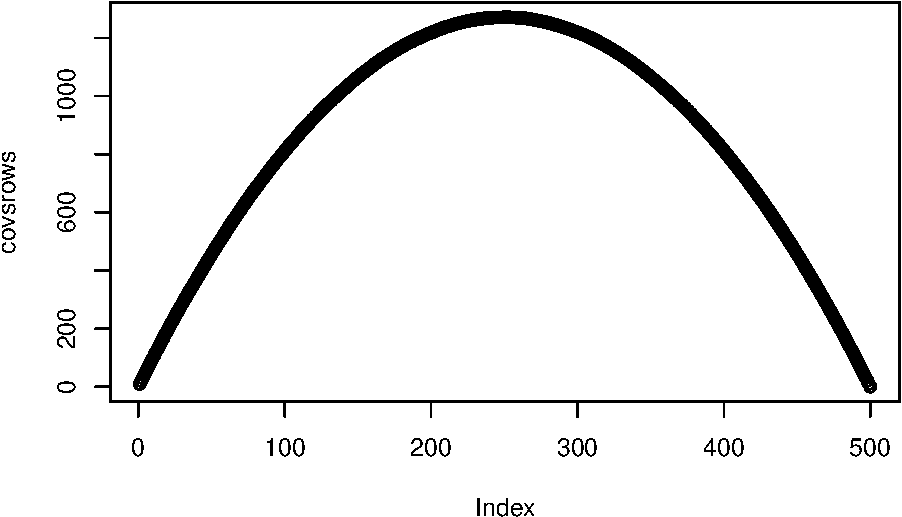
\includegraphics{./figures/unnamed-chunk-11-1.pdf}
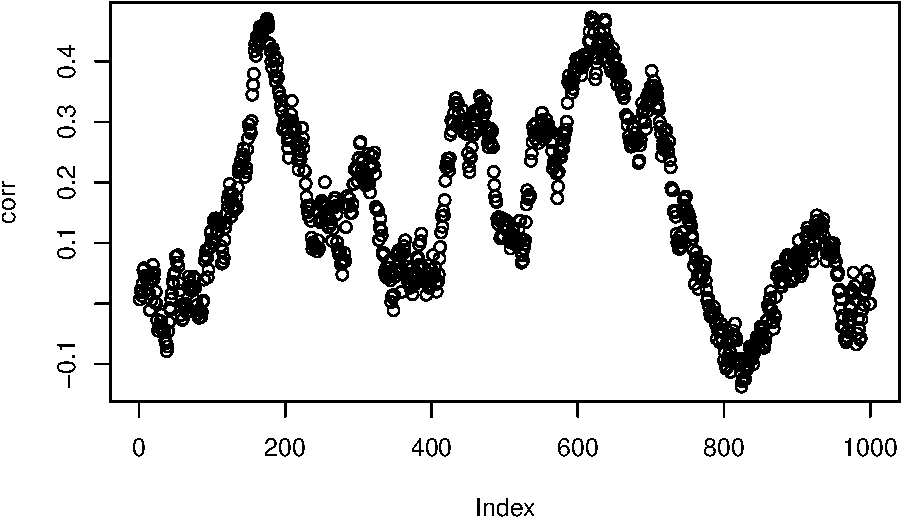
\includegraphics{./figures/unnamed-chunk-11-2.pdf}

Trying using a variable with both positive and negative values as
quantitative variable vs our binary variable

\begin{Shaded}
\begin{Highlighting}[]
\KeywordTok{simulate}\NormalTok{(}\DecValTok{1000}\NormalTok{,}\DecValTok{50}\NormalTok{,}\OperatorTok{-}\DecValTok{30000}\NormalTok{,}\DecValTok{30000}\NormalTok{)}
\end{Highlighting}
\end{Shaded}

\hypertarget{what-information-does-the-sample-covariance-provide}{%
\subsection{What information does the sample covariance
provide?}\label{what-information-does-the-sample-covariance-provide}}

We know that because the Private variable (binary variable) has only 2
possible values, its covariance with other variables is always going to
be relatively small and will not provide much information.

\newpage

\hypertarget{what-information-does-the-sample-correlation-provide}{%
\subsection{What information does the sample correlation
provide?}\label{what-information-does-the-sample-correlation-provide}}

\end{document}
